% Created 2021-08-22 dom 17:05
% Intended LaTeX compiler: pdflatex
\documentclass[11pt]{article}
\usepackage[utf8]{inputenc}
\usepackage[T1]{fontenc}
\usepackage{graphicx}
\usepackage{grffile}
\usepackage{longtable}
\usepackage{wrapfig}
\usepackage{rotating}
\usepackage[normalem]{ulem}
\usepackage{amsmath}
\usepackage{textcomp}
\usepackage{amssymb}
\usepackage{capt-of}
\usepackage{hyperref}
\usepackage{minted}
\usepackage[left=0.35in,top=0.25in,right=0.35in,bottom=0.25in]{geometry}
\usepackage[no-math]{fontspec}
\setsansfont{Linux Libertine}
\renewcommand{\familydefault}{\sfdefault}
\author{Guilherme Gomes Haetinger - \texttt{00274792}}
\date{\today}
\title{Assignment 0 - Rendering Triangles in \uline{OpenGL}}
\hypersetup{
 pdfauthor={Guilherme Gomes Haetinger - \texttt{00274792}},
 pdftitle={Assignment 0 - Rendering Triangles in \uline{OpenGL}},
 pdfkeywords={},
 pdfsubject={},
 pdfcreator={Emacs 27.2 (Org mode 9.5)}, 
 pdflang={English}}
\begin{document}

\maketitle

\noindent\rule{\textwidth}{0.5pt}

\section{Setup}
\label{sec:org651e0a6}

I had problems building the code from the Github provided source. Thus, I
adapted the source code to use my local \uline{GLEW} and \uline{GLFW3} setup. If you are to
run my code, make sure you have them installed in your lib path.

Not quite sure what the problem was, but it might have something to do with the
compilation of the \texttt{vermilion} files.

\section{Code}
\label{sec:org7d1dbd1}

As a task, we also had to change how the triangles were built, removing one of
them from the final image and making the remaining one colorful. To do so, we
have to add in a few enums:

\begin{minted}[]{cpp}
enum Buffer_IDs { ArrayBuffer, ColorBuffer, NumBuffers };
enum Attrib_IDs { vPosition = 0, vColor = 1 };
\end{minted}

Also, as we remove one of the triangles, we also need to define a color array,
leaving us with:

\begin{minted}[]{cpp}
GLfloat vertices[NumVertices][2] = {{-0.90f, -0.90f}, {0.85f, -0.90f}, {-0.90f, 0.85f}};
GLfloat colors[NumVertices][3] = {{1.0f, 0.0f, 0.0f}, {0.0f, 1.0f, 0.0f}, {0.0f, 0.0f, 1.0f}};
\end{minted}

Once we have them defined, we bind the \texttt{ColorBuffer}, set its storage to the
size of the array and enable it.

\begin{minted}[]{cpp}
glBindBuffer(GL_ARRAY_BUFFER, Buffers[ColorBuffer]);
glBufferStorage(GL_ARRAY_BUFFER, sizeof(colors), colors, 0);

glVertexAttribPointer(vColor, 3, GL_FLOAT, GL_FALSE, 0, 0);
glEnableVertexAttribArray(vColor);
\end{minted}

All this data will go to the vertex shader and can be interpolated onto separate
fragments processed by the fragment shader. So, the first thing we do is to
receive and send a color \texttt{vec3} in the vertex shader:

\begin{minted}[]{glsl}
#version 400 core

layout( location = 0 ) in vec4 vPosition;
layout( location = 1 ) in vec4 vColor;

out vec4 color;

void
main()
{
    gl_Position = vPosition;
    color = vColor;
}
\end{minted}

And the fragment shader receives and forwards it.

\begin{minted}[]{glsl}
#version 450 core

in vec4 color;
out vec4 fColor;

void main()
{
    fColor = color;
}
\end{minted}

\section{Results}
\label{sec:orgf5e9d95}

\begin{figure}[htbp]
\centering
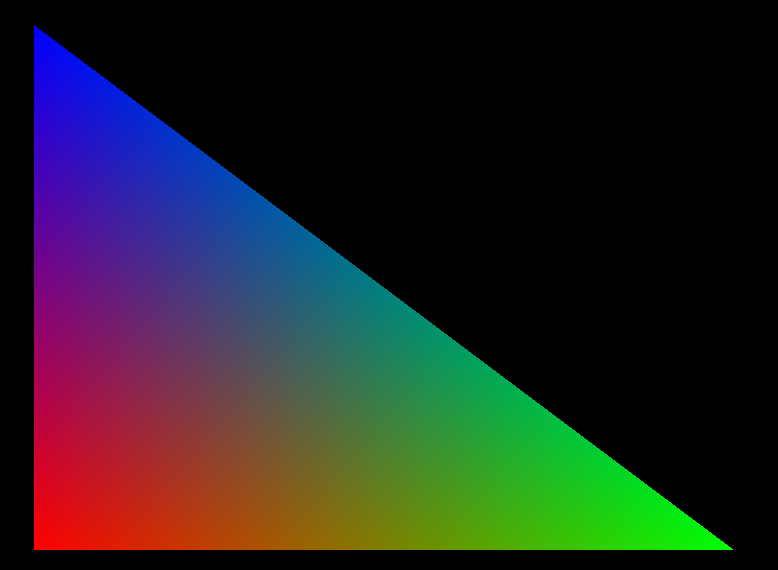
\includegraphics[width=.9\linewidth]{./triangle.png}
\caption{Colorful Triangle}
\end{figure}
\end{document}
